\subsection*{Aufgabe 17}
Gegeben ist die Dispersionsrelation für ein fcc-Gitter:
\begin{align}
\label{eq-disp}
  E(k) = E'_\alpha - 4\;|A| \left(\cos\frac{k_x a}{2}\cos\frac{k_y a}{2} +
    \cos\frac{k_y a}{2}\cos\frac{k_z a}{2} + \cos\frac{k_z a}{2}\cos\frac{k_x a}{2} \right)
\end{align}

\subsubsection*{a)}
\begin{wrapfigure}[11]{R}{8cm}
  \centering
  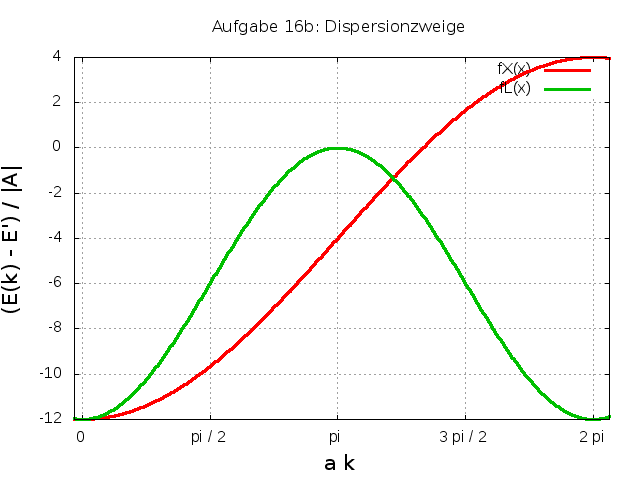
\includegraphics[width=7.5cm]{aufgabe16b.png}
\label{bild16b}
\end{wrapfigure}
Im LCAO-Modell beschreibt das Austauschintegral A den Overlap der Wellenfunktion
eines (Valenz-)Elektrons mit den Wellenfunktionen der (Valenz-)Elektronen benachbarter
Atome. Daraus resultiert eine Aufspaltung der Bänder; diese ist propotional zu A
und einem Geometriefaktor (runde Klammer in obiger Formel) und ist dadurch
auch abhängig von $\vec k$.
\newline
\subsubsection*{b)}
\begin{itemize}
\item[$\Gamma$ X:]
  In $\Gamma$X-Richtung ist $k_y = k_z = 0$, sei $k:= k_x$, dann wird \eqref{eq-disp}
  wegen $\cos(0) = 1$:
\begin{align*}
    E(k) = E'_\alpha - 4\;|A| \left(1 + 2 \cos\frac{k a}{2} \right)
\end{align*}
Siehe rote Kurve fX im Plot. Da $\cos(k)$ Werte zwischen -1 und +1 annehmen kann
ergibt sich eine Bandbreite $B = 16\;|A|$.
\item[$\Gamma$ L:]
  In $\Gamma$L-Richtung ist $k_x = k_y = k_z =: k$, dann wird \eqref{eq-disp}:
\begin{align*}
    E(k) = E'_\alpha - 4\;|A| \left(3 \cos^2\frac{k a}{2} \right)
\end{align*}
Siehe grüne Kurve fL im Plot. Da $\cos^2(k)$ Werte zwischen 0 und +1 annehmen kann
ergibt sich eine Bandbreite $B = 12\;|A|$.
\end{itemize}

\subsubsection*{c)}
Die im Aufgabenblatt rot eingezeichneten Basisvektoren des zweidimensionalen
hexagonalen Gitters haben die Koordinaten
\begin{align*}
  \vec a_1 = a \cdot \begin{pmatrix} 1 \\ 0 \\ 0 \end{pmatrix} \;; \qquad
  \vec a_2 = a \cdot \begin{pmatrix} \cos(120^\circ)\\ \sin(120^\circ)\\ 0\end{pmatrix} =
  a \cdot \begin{pmatrix} -\frac{1}{2}\\\frac{1}{2} \sqrt{3}\\ 0 \end{pmatrix}
\end{align*}
(Zur Berechnung der inversen Gittervektoren ein kurzer Ausflug in drei Dimensionen.)
Damit wird $ | \vec a_1 \times \vec a_2 | = \frac{1}{2} \sqrt{3} a^2$ und für die
Basisvektoren im inversen Gitter ergibt sich:
\begin{align*}
\vec b_1 =  \frac{2 \pi}{\frac{1}{2} \sqrt{3} a^2} (\vec a_2 \times \vec e_3 ) =
  \frac{2 \pi}{a} \begin{pmatrix} 1 \\ 1 / \sqrt{3} \\ 0 \end{pmatrix} \;; \qquad
  \vec b_2 =  \frac{2 \pi}{\frac{1}{2} \sqrt{3} a^2} (\vec e_3 \times \vec a_1) =
  \frac{2 \pi}{a} \begin{pmatrix} 0 \\ 2 / \sqrt{3} \\ 0 \end{pmatrix}
\end{align*}
Man verifiziert leicht: $\vec a_i \cdot \vec b_j = 2 \pi \delta_{ij}$. Jetzt wieder
zweidimensional: Im Real-Raum hat ein Atom im Koordinatenursprung 6 nächste Nachbarn
mit den Koordinaten $R_n\;;\;n = 1, \cdots , 6$ im Gegen-Uhrzeigersinn:
\begin{align*}
\left\lbrace R_n\right\rbrace &= \left\lbrace
 \vec a_1,\; \vec a_1 + \vec a_2,\; \vec a_2, -\vec a_1,\; -\vec a_1 - \vec a_2,\; - \vec a_2
  \right\rbrace
\intertext{Für die Dispersion gilt im LCAO-Modell mit der "`nächste-Nachbarn-Annäherung"':}
\epsilon(\vec k) &= \epsilon'_\alpha + |A| \sum_{n = 1}^6 \mathrm e^{i \vec k \vec R_n}
\intertext{Für das unterste Band ist $\vec k =  \frac{a}{2 \pi}\left(1 \cdot k_x \vec b_1 + 1 \cdot k_y \vec b_2 \right)$, damit wird}
\left\lbrace \vec k \vec R_n \right\rbrace &= \left\lbrace
  a k_x\;, \;a k_x + a k_y\;, \;a k_y\;, \;-a k_x\;, \;-a k_x- a k_y\;, \;-a k_y \right\rbrace \\
\sum_{n = 1}^6 \mathrm e^{i \vec k \vec R_n} &=
\end{align*}

